%!TEX root = Slic3r-Manual.tex
\section{Travailler avec les mod\`eles 3D}
\label{sub:working_with_models}
\index{models}
\index{mod\`eles 3D}

Il reste encore une \'etape avant la premi\`ere impression: obtenir un mod\`ele 3D et le "trancher".

\subsection{Formats de Mod\`eles 3D} % (fold)
\label{sub:model_formats}
\index{STL}
\index{AMF}
\index{OBJ}

Slic3r accepte les types de fichiers suivants :

\begin{itemize}
	\item Les fichiers ST\'er\'eolithographique (STL) peuvent provenir d'une grande vari\'et\'e de sources et sont maintenant un standard de facto dans l'impression 3D. Les fichiers d\'ecrivent simplement la g\'eom\'etrie de la surface d'un objet 3D sans aucune information suppl\'ementaire (comme la couleur ou la mati\`ere), et c'est cette simplicit\'e qui a probablement fait le format omnipr\'esent.
	\item Le type de fichier Wavefront OBJ est un format ouvert utilis\'e \`a l'origine dans une application d'animation de Wavefront Technologies, mais a depuis \'et\'e adopt\'ee par la communaut\'e de la mod\'elisation 3D. Il est similaire au format STL.
	\item Le format de fichier AMF (Additive Manufacturing File Format) a \'et\'e d\'evelopp\'e en r\'eponse au caract\`ere limit\'e du format STL. En plus de d\'ecrire la g\'eom\'etrie du mod\`ele 3D, il peut \'egalement d\'ecrire les couleurs et les mat\'eriaux, ainsi que des attributs plus complexes, tels que les m\'elanges d\'egrad\'es et de multiples arrangements d'objets (constellations). Alors que le format est consid\'er\'e comme un standard, il reste \`a \^etre largement adopt\'ee dans le milieu de la machine 3D.
\end{itemize}
% subsection model_formats (end)

\subsection{Trouver des Mod\`eles 3D} % (fold)
\label{sub:finding_models}
\index{models!finding}
\index{mod\`eles!trouver}

Les fichiers de mod\`ele 3D peuvent provenir d'un d\'ep\^ot en ligne, tels que Thingiverse\footnote{\url{http://www.thingiverse.com}} ou GrabCAD\footnote{\url{http://grabcad.com}}, ou \^etre cr\'e\'es \`a partir d'un programme de CAO, comme FreeCAD\footnote{\url{http://sourceforge.net/projects/free-cad}}, Sketchup\footnote{\url{http://www.sketchup.com}}, ou OpenSCAD\footnote{\url{http://www.openscad.org}}, ou un outil de CAO en ligne tels que Shapesmith\footnote{\url{http://shapesmith.net}}.

Vous souhaitez peut-\^etre afficher les fichiers avant de trancher et il y a beaucoup d'applications disponibles, dont l'un est Meshlab\footnote{\url{http://www.meshlab.org}} - un outil complet pour la visualisation et la manipulation des fichiers 3D.

\begin{figure}[H]
\centering
\includegraphics[keepaspectratio=true,width=0.75\textwidth]{working_with_models/shapesmith.png}
\caption{Outil de CAO en ligne Shapesmith.}
\label{fig:shapesmith}
\end{figure}

% subsection working_with_models (end)


\subsection{Utiliser la Surface de Travail} % (fold)
\label{sub:working_with_plater}
\index{Plater}
\index{Surface de Travail}
Slic3r dispose d'un outil, appel\'e Plater, qui permet \`a un ou plusieurs mod\`eles d'\^etre charg\'es et dispos\'es avant d'\^etre "tranch\'es".

\begin{figure}[H]
\centering
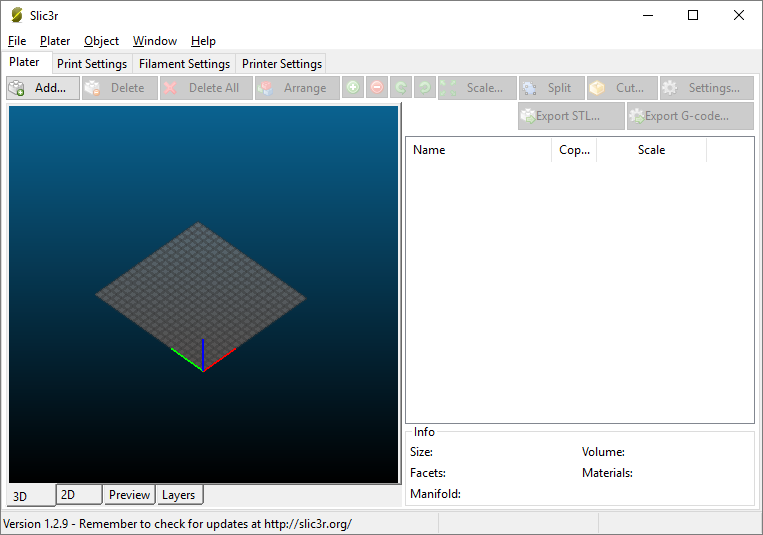
\includegraphics[keepaspectratio=true,width=1\textwidth]{working_with_models/plater.png}
\caption{Surface de Travail}
\label{fig:plater}
\end{figure}


Une fois que vous avez acquis un mod\`ele, faites-le glisser sur l'onglet "Plater" (ou utilisez le bouton Add(Ajouter) dans le coin sup\'erieur gauche) pour le charger dans Slic3r. Dans la figure ci-dessous, la traditionnelle Minimug RepRap\footnote{\url{http://www.thingiverse.com/thing:18357}} est chargée, et est vue de dessus. L'anneau autour du modèle est une jupe - un seul périmètre, à quelques millimètres du modèle, qui est extrudé en premier. Ceci est utile pour s'assurer que la matière plastique est fluide à partir de la buse lorsque le modèle commence à être imprimé.

\begin{figure}[H]
\centering
\includegraphics[keepaspectratio=true,width=0.75\textwidth]{working_with_models/minimug_model.png}
\caption{Le Mod\`ele Minimug.}
\label{fig:minimug_model}
\end{figure}

\begin{figure}[H]
\centering
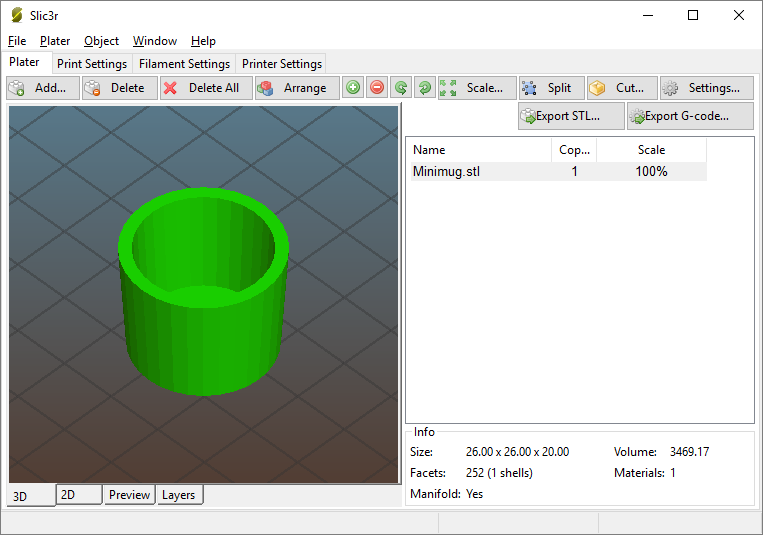
\includegraphics[keepaspectratio=true,width=1\textwidth]{working_with_models/plater_model_loaded.png}
\caption{Fichier STL charg\'e.}
\label{fig:plater_model_loaded}
\end{figure}

Le mod\`ele peut \^etre repositionn\'e en le d\'eplaçant sur la repr\'esentation du lit \`a gauche de l'\'ecran. Notez que les dimensions du lit doivent correspondre \`a votre imprimante, telles qu'elles sont donn\'ees lors de la configuration initiale ci-dessus.

Sur le c\^ot\'e droit il y a la liste des fichiers actuellement charg\'es. Les boutons situ\'es en haut de la liste de fichier vous permettent d'organiser les mod\`eles.
\begin{itemize}
	\item \textbf{More/Less (plus/moins)}  - R\'egle le nombre de copies qui doit \^etre imprim\'e.
	\item \textbf{45°/Rotate (45°/rotation)}  - Fait pivoter le mod\`ele s\'electionn\'e autour de l'axe Z, soit de 45 ° dans le sens horaire ou anti-horaire, ou par une valeur donn\'ee.
	\item \textbf{Scale (\'echelle)}  - Augmenter ou diminuer la taille du mod\`ele imprim\'e.
	\item \textbf{Split (dissocier)}  - Divise un mod\`ele qui se compose de plus d'une partie en ses parties constituantes, ce qui permet \`a chacune d'\^etre agenc\'ee individuellement.
\end{itemize}


Les boutons en haut \`a gauche, vous permettent d'ajouter, de supprimer, d'auto-organiser, ou d'exporter les mod\`eles.
\begin{itemize}
	\item \textbf{Add (Ajouter)}  - Ouvre une bo\^ite de dialogue pour ajouter un mod\`ele \`a la surface de travail, c'est une alternative gliss\'e/d\'epos\'e du fichier sur la surface de travail.
	\item \textbf{Delete/Delete All (Supprimer/Tout supprimer)}  - Retirer un ou tous les mod\`eles de la surface de travail.
	\item \textbf{Autoarrange}  - Essaye d'organiser les mod\`eles pour obtenir l'agencement optimal.
	\item \textbf{Export G-code}  - D\'emarre le "tranchage" du mod\`ele, et produit un fichier G-code.
	\item \textbf{Export STL}  - Sauvegarde un ensemble de mod\`ele de la surface de travail dans un fichier STL unique.
\end{itemize}


L'epace de travail plater est divisé en quatre vue sélectionable par des onglets au bas de la vue

La vue par défaut est la vue 3D, le deuxième onglet permet de travailer sur la vue de dessus en 2D

\begin{figure}[H]
\centering
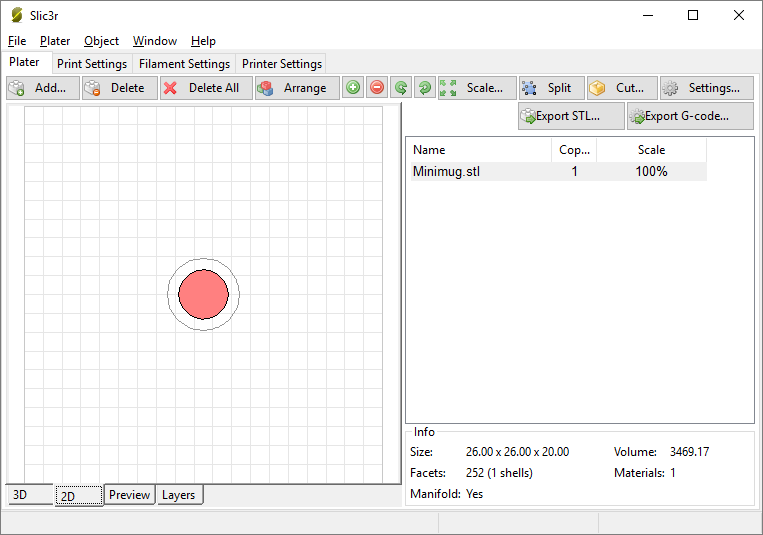
\includegraphics[keepaspectratio=true,width=1\textwidth]{working_with_models/plater2d.png}
\caption{Surface de Travail en 2D}
\label{fig:plater2d}
\end{figure}
L'onglet preview affiche la vue de pévisualisation en 3D de l'impression, le filament extrudé est représenté sur cette vue. Le curseur permet de faire d\'efiler les couches.

\begin{figure}[H]
\centering
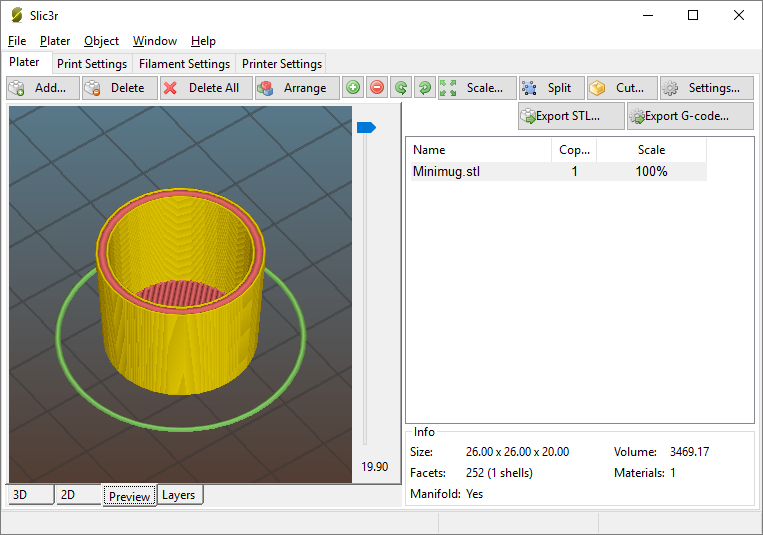
\includegraphics[keepaspectratio=true,width=1\textwidth]{working_with_models/platerpreview.png}
\caption{Prévisualisation en 3D}
\label{fig:platerpreview}
\end{figure}
L'onglet layer affiche la vue 2D le chaques couches, le curseur sur la droite permet de faire de selectionner la couche \`a visualiser.

\begin{figure}[H]
\centering
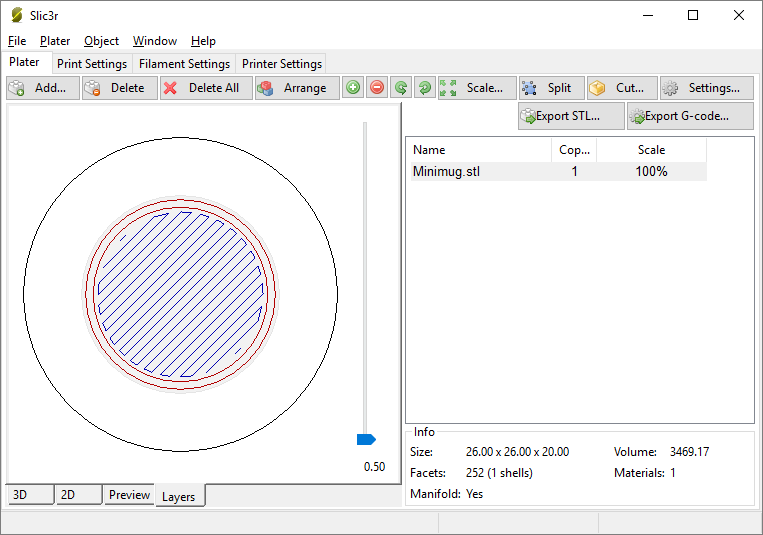
\includegraphics[keepaspectratio=true,width=1\textwidth]{working_with_models/platerlayer.png}
\caption{Prévisualisation des couches}
\label{fig:platerlayer}
\end{figure}


% subsection working_with_plater (end)

\subsection{R\'eparer les fichiers STL} % (fold)
\label{sub:cleaning_stls}
\index{STL!cleaning}
\index{STL!r\'eparer}
Si le maillage 3D d\'ecrit dans le mod\`ele contient des trous, ou les bords ne sont pas align\'es (connu comme \'etant non-manifold), Slic3r peut avoir des probl\`emes pour le traiter. Slic3r va tenter de r\'esoudre les probl\`emes, mais certains probl\`emes sont hors de sa port\'ee. Si l'application se plaint que le mod\`ele ne peut pas \^etre "tranch\'e" correctement alors il y a plusieurs options possibles: voir le chapitre sur la R\'eparation des mod\`eles.

% subsection cleaning_stls (end)
